\documentclass[letter]{report}
\usepackage{epsfig}
\usepackage{amssymb}

\pagestyle{empty}

\title{ {\LARGE\bf \emph{DRAFT} \\
        Mesquite User's Guide\\
                 \emph{DRAFT} }}

\author{Patrick Knupp, Lori Freitag, Darryl Melander, Mike Brewer \\
The Sandia National Laboratories \\
Albuquerque NM USA \\
and \\
Thomas Leurent \\
Argonne National Laboratory \\
Argonne, IL 60490 USA}

\date{}

\begin{document}

\maketitle

\tableofcontents

\listoffigures

\listoftables

\chapter{Introduction to Mesh Quality Improvement} 

\section{General Overview}

Mesh quality has been shown to be critical for solution accuracy and
efficiency in the solution of PDE-based applications.  However, it can
be negatively impacted during many stages of the mesh generation
process from de-featuring CAD models to post-processing via a smoothing
scheme to mesh adaptivity. At any stage after a mesh is created, its
quality can be improved by techniques such as node point movement and
topology modification.  There are a number of techniques that have
been developed for mesh improvement ranging from simple Laplacian smoothing
\cite{F88} to more sophisticated algorithms such as Winslow smoothers
for structured meshes (for example, \cite{winslow}), the numerical
optimization methods and topology modification schemes recently
developed for unstructured meshes (for example, \cite{Opt-MS,Kn00,FrKn01,
FeasNewt,bjoe:swap,bjoe:chain-swap,es92}).

Mesquite (Mesh Quality Improvement Toolkit) is designed to provide a
stand-alone, portable package for mesh quality improvement which
includes a comprehensive suite of these algorithms.  It is designed in
such a way that they can be applied to many different mesh element
types and orders and referenced to both isotropic and anisotropic
ideal elements.  The successful completion of Mesquite will provide a
robust and effective mesh improvement toolkit to the broader
scientific community.  This will allow both mesh generation
researchers and application scientists to benefit from the latest
developments in mesh quality control and improvement.

The goals of this user's manual are to
\begin{itemize}
\item provide a vision for Mesquite (what it is and what it will become),
\item cover both novice and expert users. The novice should know how to
download, compile and use the simplified Mesquite user's interface
after reading a small percentage of the guide. More 
advanced concepts are included later in the text.
\item provide practical instructions on using Mesquite API, compiling,
linking, TSTT interface,
\item provide insight into the mathematical concepts and optimization 
algorithms which are the heart of the Mesquite mesh quality improvement 
toolkit
\end{itemize}

\section{Mesh Improvement Goals}

{\it Why have different mesh improvement goals? What are they (shape,
untangle, alignment, morph, etc.). Improvement goals currently
supported (shape, untangle).  }

\section{The Mesquite Philosophy}

{\it 
The Hippocratic oath: we will do no harm (can we do an undo or
should the user keep track of the original mesh?).  What are the
boundaries of Mesquite?  What it is not going to do. What do we mean
by a mesh quality improvement algorithm. Including the best known
algorithms for a particular goal (not just a collection of hacked
tools). Provides both a useful tool that is easy to use for
application scientists and is extensible to provide a platform for
mesh quality improvement research. Give an example API file (script for
Laplace smoothing - novice). Show the expert view of the
world. Readers can use script to build from. Use example to help
explain our philosophy. 
}

\section{The Mesquite Vision}

Mesquite design goals are derived from a mathematical framework and
are focused on providing a versatile, comprehensive, effective,
inter-operable, and efficient library of mesh quality improvement
algorithms that can be used by the non-expert and extended and
customized by experts.  In this section we highlight the current
status of Mesquite in several of our design goal areas.

{\bf Mathematical Framework.}  Mesquite design is based on a currently
evolving, but rigorous mathematical framework that poses the mesh
quality improvement, node-movement problem as an optimization problem.
That is, suppose a mesh $M$ contains $n$ vertices, $v_i$, and $k$
elements, $e_i$.  Then the quality of each element or vertex is given
as a general function $q_i ( {\bf x} )$ of the coordinates of the
vertex locations.  The index $i$ ranges from 1 to $n$ or 1 to $k$
depending on whether a vertex-based or element-based metric is chosen.
A mesh quality objective function ${\cal F} = f(q_i({\bf x} ))$ for
$i=1,\cdots,n_s$ or $i=1,\cdots,k_s$ is formed to give an overall
measure of mesh quality where $n_s$ and $k_s$ are the number of
vertices or elements in a mesh sub-domain needing improvement,
respectively.  Mesquite is designed to solve the minimization problem
${\rm min}~{\cal F}$ for a broad collection of quality metrics $q_i$
and objective functions ${\cal F}$.

{\bf Versatile and Comprehensive.}  Mesquite works on structured,
unstructured, and hybrid meshes in both two and three dimensions. The
design permits improvements to meshes composed of triangular,
tetrahedral, quadrilateral, and hexahedral elements. Prismatic,
pyramidal, and polyhedral elements can be easily added.  
%Mesquiteincorporates the best quality improvement methods to solve 
%discrete objective functions composed of mesh quality metrics. 
It currently incorporates only methods for node movement; plans for 
topology modification and hybrid improvement strategies lie in the future.
Node movement strategies include both local patch-based iteration
schemes for one or a few free vertices and global objective functions
which improve all vertices simultaneously.  Mesquite will be
applicable to both adaptive and nonadaptive meshing and to both low-
and high-order discretization schemes, but currently works with
non-adaptive meshes containing linear elements.

{\bf Effective.}  Mesquite uses state-of-the-art algorithms and
metrics to guarantee improvement in mesh quality.  Because the
definition of mesh quality is application specific, we provide quality
metrics that allow the user to untangle meshes, improve mesh
smoothness, element size, and shape. In the future these metrics will
be referenced to permit non-isotropic smoothing and adaptivity. The
software is easily customizable, enabling users to insert their own
quality metrics, objective functions, and algorithms and also provides
mechanisms for creating combined approaches that use one or more
improvement algorithms.

{\bf Inter-operable.}  To ensure that Mesquite is inter-operable with a
large number of mesh generation packages, we will use the common
interfaces for mesh query currently under development by the TSTT
center.  These interfaces provide uniform access to mesh geometry and
topology and will be implemented by all TSTT center software including
several DOE-supported mesh generation packages.  We are working with
the TSTT interface design team to ensure that Mesquite has efficient
access to mesh and geometry information through strategies such as
information caching and agglomeration.  We are also participating in
the design of interfaces needed to support topological changes
generated by mesh swapping and flipping algorithms and to constrain
vertices to the surface of a geometrical model.

%{\bf Robust.} Mesquite guarantees that there will be no degradation to
%mesh quality as measured by the objective function and quality metric
%used for improvement.  To achieve this goal, we use sound software
%engineering principles and robust numerical algorithms.  A
%comprehensive suite of test problems and a unit testing framework have
%been developed to verify the correct execution of the code.

{\bf Efficient.}  The outer layers of Mesquite use 
object-oriented design in C++ while the inner kernels use
optimizable coding constructs such as arrays and inlined
functions.  To ensure efficient use of computationally intensive
optimization algorithms, we employ inexpensive smoothers, such as
Laplacian smoothing, as ``preconditioners'' for the more expensive
optimization techniques.  In addition, mesh culling algorithms can be
used to smooth only those areas of the mesh that require improvement.
Considerable attention has been devoted to understanding and
implementing a variety of termination criteria that can be used to
control the computational cost of the optimization algorithms.

{\it In core to applications, not just a preprocessing step.}

\chapter{Basic Mesquite Usage}

\section{Downloading Mesquite}

\subsection{System Requirements}
TODO:  List the supported platforms (Lin, SGI, Sun, etc.?), the required
software (makedepend, gmake, Babel, etc.?), and any related information.
\subsection{Acquiring the Necessary Code/Libraries}
TODO:  How and where Mesquite, AOMD, CppUnit, (MDB), etc. can be
acquired... with appropriate acknowledgments.

\section{Compiling and Linking Mesquite}
\label{sec:compiling}
\begin{verbatim}
TODO:  Software dependencies, compiling AOMD, TSTT interfaces
(need the .h file), other (gmake, makedepend)?  
Makefiles (examples that link Mesquite to an 
application code). Compiler flags and options (debugging, profiling). 
Platforms supported. Optional functionalities (debugging, profiling, 
error handling).
\end{verbatim}

Having acquired the Mesquite source code, the user can perform the
following steps which outline the process for compiling the code and
creating the library, `libmesquite.a'. Here is the fastest way to compile Mesquite:
\begin{enumerate}
\item While in the main directory (typically, .../mesquite/), type
`./configure'.  This will create the file Makefile.customize with a default configuration
for your platform.
\item Type gmake, this will compile the library lib/libmesquite.a
\item To compile, one of the test, stay in the main directory (mesquite/) and type 
for example 'gmake testSuite/test\_1/main'. You can also use 'gmake all\_tests' .
\end{enumerate}
If the above worked, you are done. Mesquite compiled successfully. 

If the above method did not work for your system, you will have to modify the file
Makefile.customize that contains the platform specific tools and settings to be used 
while compiling Mesquite. In the remainder of this section, we
will  list some of the specific variables which
may need to be modified before Mesquite will compile correctly.
This can be done in two manners: you can use the configure
script options (you can also access those options and
others by typing './configure --help'), or you can edit
Makefile.customize directly.

\subsection{Configure Options.}  \label{config_options}

Those options can be given to the configure script through the command line, for example the C headers
option would be given by typing \texttt{./configure --with-c-headers=yes} in the \texttt{mesquite/} directory.

\begin{description}
\item \texttt{--with-c-headers=yes} Uses the deprecated C style for headers:
  will use headers like \texttt{<iostream.h>} and \texttt{<math.h>}
  instead of the new C++ style \texttt{<iostream>} and \texttt{<cmath>}. This might make older
  compilers find those headers. With newer compilers, you will get a warning for using that option.
\item \texttt{--with-makedepend=EXECUTABLE} Location of alternative makedepend program:
Give the full path:  --with-makedepend='/usr/local/bin/makedepend'
\item \texttt{--with-archiver=EXECUTABLE} Location of alternative archiver (default is 'ar ru'):
Give the full path: --with-archiver='/usr/local/bin/ar' . If options are needed, we advise to
create a shell script pointed to by that option. The shell script would contain only one line: the
archiver and its options. 
\item \texttt{--with-cc=EXECUTABLE} Location of alternative C compiler:
Give the full path: --with-cc='/usr/local/gcc/bin/gcc'
\item \texttt{--with-cPP=EXECUTABLE} Location of alternative c++ compiler:
Give the full path:  --with-cPP='/usr/local/gcc/bin/g++'
\item \texttt{--with-aomd=AOMD\_LIB} Location of aomd library (optional):
Give the full path: --with-aomd='/.../libaomd.so'or check out the library from the
TSTT web pages.
\item \texttt{--with-dox=EXECUTABLE} Location of doxygen:
Give the full path: --with-dox='/usr/local/bin/doxygen'
\end{description}

\subsection{Makefile Variables.}  \label{mes_vars_and_defs}

The following is a list of variables used in Mesquite's Makefile
structure to allow for customization of the compilation process.
Most of the provided examples come directly from Mesquite's default
Linux setup. If you decided not to use the configure script and its options (previous paragraph),
you can edit Makefile.customize directly. Here are the variables and their meaning.
\begin{enumerate}

\item Tools used by Mesquite:
  \begin{description}
  \item[ARCHIVER] defines the command to call the archiver\\
    	({\it e.g.,} ARCHIVER = ar ru).
  \item[CXX] defines the command to call the compiler\\
	({\it e.g.,} CXX = g++).
  \item [LINKER] defines the command to call the linker\\
	({\it e.g.,} LINKER = \$\{CXX\}).
  \item[MAKEDEPEND] defines the command to call makedepend\\
	({\it e.g.,} MAKEDEPEND = makedepend).
  \end{description}

\item Compilation flags and variables:
  \begin{description}
  \item[AOMD\_FLAG]
  \item[CXX\_FLAGS]
  \item[DEBUG\_FLAG] defines the flags to be used to compile the Mesquite
	with the desired levels of debug information, optimization, and
	warning statements\\
	({\it e.g.,} DEBUG\_FLAG = -g -Wno-deprecated).
  \item[DEPEND\_FLAGS]
  \item[LD\_FLAGS]
  \item[STD\_INCLUDE\_FLAG] defines certain global definitions that
	tell the compiler which types of header files to include. The configure script has the
	option \texttt{--with-c-headers} to help set this variable.
 	Essentially, the two options are USE\_STD\_INCLUDES and
	USE\_C\_PREFIX\_INCLUDES.  With USE\_STD\_INCLUDES defined
	Mesquite will include the standard header files.  For example,
	`list' will be included instead of `list.h'.  With
	USE\_C\_PREFIX\_INCLUDES defined, Mesquite will include the
	`c-prefixed' header files.  For example, `cmath' will be
	included instead of `math.h'.  \\
	({\it E.g.,} STD\_INCLUDE\_FLAG = -DUSE\_STD\_INCLUDES\\
	-DUSE\_C\_PREFIX\_INCLUDES).
  \end{description}
\item Directories:
  \begin{description}
  \item[AOMD\_LIB\_DIR] is an optional variable which can be set
	to hold the location of the AOMD library if Mesquite will
	be linked to AOMD\\
	({\it e.g.,} AOMD\_LIB\_DIR = \$\{MSQ\_BASE\_DIR/external/AOMD/lib\}).
  \item[EXODUS\_LIB\_DIR] is an optional variable used to hold the
	location of the Exodus II library, an external library needed
	by MDB.  This library is not needed if Mesquite is not being
	linked to MDB.
	({\it E.g.,} EXODUS\_LIB\_DIR = \$\{MSQ\_BASE\_DIR\}/external/exodus/lib).
  \item[MDB\_LIB\_DIR] is another optional variable which can be set
	to hold the location of the MDB library if Mesquite will
	be linked to MDB\\
	({\it e.g.,} MDB\_LIB\_DIR = \$\{MSQ\_BASE\_DIR\}/external/MDB/lib).
  \item[MSQ\_BASE\_DIR] holds the name of the main Mesquite directory.
	Generally, the default value for this variable will be correct.\\
	(The default value is `MSQ\_BASE\_DIR = .').
  \end{description}
\item TSTT linking information:
\begin{description}
  \item[AOMD\_TSTT\_LINK] is an optional variable that holds the
	information needed by the linker to link the AOMD to Mesquite\\
	({\it e.g.,} AOMD\_TSTT\_LINK = -L\$\{AOMD\_LIB\_DIR\} -lAOMD -lm).
  \item[MDB\_TSTT\_LINK] is an optional variable that holds the
	information needed by the linker to link the MDB to Mesquite\\
	({\it e.g.,} MDB\_TSTT\_LINK = -L\$\{MDB\_LIB\_DIR\} -lMDB -lm).
  \item[TSTT\_LINK] holds the information used by the LINKER to link
	the TSTT implementation to Mesquite \\
	({\it e.g.,} TSTT\_LINK = \$\{AOMD\_TSTT\_LINK\}).
\end{description}
\end{enumerate}

\section{Short Tutorial}

In this section, we will write a Mesquite driver in order to improve the quality of a test
mesh. This tutorial section is aimed at giving you a feel for Mesquite: \emph{this section is not where to look
for detailed information}. In particular, informations on loading a particular mesh format, or
interacting through a particular mesh interface, and details of the API classes
are not given in this section.

At first, we will write a small program using Mesquite's simplified API, or wrappers, in order to show the
fastest way to get Mesquite running on a mesh. The concept of the wrappers, as well as the different
wrappers available, are described in section \ref{sec:wrappers}. We will then set up a more customized mesh
improvement tool through the mesquite low-level API, described in section \ref{sec:}

\subsection{Tutorial File Template}
\label{sec:tutfile}

In order to create and link a driver code, the Mesquite library must have been compiled, as per the
instructions of section \ref{sec:compiling}. For this tutorial, we will edit the file
\texttt{testSuite/tutorial/tutorial.cpp}, which contains the following template:
\begin{verbatim}
#include "Mesquite_all_headers.hpp"
using namespace Mesquite;
int main(int argc, char* argv[])
{
  MsqError err;
  
  
}
\end{verbatim}
Mesquite provides a convenient header file \texttt{include/Mesquite\_all\_headers.hpp} that includes
all Mesquite headers. This is the easiest way to deal with the include directives although it is likely to slow
down your Mesquite compilation.
All Mesquite classes are part of the \texttt{Mesquite} namespace. Be aware that general mesh interfaces
classes usually have their own namespace. The \texttt{MsqError} class is an error object passed to 
certain function calls (see section \ref{sec:}), its value is checked after the functions calls with
the macro \texttt{MSQ\_CHKERR(...)}.

Although the code above does not perform any action, we can compile from the main directory
(\texttt{mesquite/}) it with the command 
\begin{verbatim}
gmake testSuite/tutorial/tutorial
\end{verbatim}

\subsection{Loading a Test Mesh}

Here we want to improve one of the test meshes distributed with Mesquite. Those meshes are in
the very readable but inefficient VTK format. You can open one of the ASCII files in
\texttt{mesquite/meshFiles/...} and check it out for yourself.
To load a VTK test mesh in Mesquite, instantiate the Mesquite mesh database object,
\texttt{MeshImpl}\footnote{Note that if you have your own mesh
database running, you should use the interfaces described in section \ref{sec:meshes}.}, 
and use the \texttt{read\_vtk} function by adding those lines to the file
template described in \ref{sec:tutfile}.
\begin{verbatim}
  Mesquite::MeshImpl *my_mesh = new Mesquite::MeshImpl;
  my_mesh->read_vtk("../../meshFiles/2D/VTK/square_quad_10_rand.vtk", err); 
  MSQ_CHKERR(err);
\end{verbatim}
You now need to add the mesh to a MeshSet, an object that can regroup several contiguous meshes to
improve them all at once:
\begin{verbatim}
  Mesquite::MeshSet mesh_set;
  mesh_set.add_mesh(my_mesh, err); MSQ_CHKERR(err);
\end{verbatim}
At this point, the MeshSet might also need some information concerning the mesh geometry. Mesquite
deals automatically with all types of supported elements, including hybrid meshes, but some meshes
require the geometry information: for example when improving a surface mesh, the user should tell
the MeshSet which surface the vertices are constrained to. In particular, all 2D meshes need to
specify some geometry constraints, since Mesquite is inherently a 3D code. 
The details are explained in section
\ref{sec:geometry}; here we show how to set the geometry of a planar 2D mesh, defined by a point and
a normal, on the MeshSet: 
\begin{verbatim}
  Vector3D normal(0,0,1);
  Vector3D point(0,0,5);
  PlanarDomain my_mesh_plan(normal, point, my_mesh);
  mesh_set.set_domain_constraint(&my_mesh_plan);
\end{verbatim}

Note that Mesquite also provides a function to write a mesh file in VTK format, given a \texttt{MeshImpl}
object: 
\begin{verbatim}
  my_mesh->write_vtk("original_mesh",err); MSQ_CHKERR(err);
\end{verbatim}


\subsection{Improving the Mesh with a Wrapper Class}
The simplest way to launch a Mesquite mesh quality improvement procedure is to use one of the
wrapper classes described in section \ref{sec:wrappers}. Here, we will instantiate the
\texttt{ShapeImprovement} and run it over the MeshSet we created earlier. Mesquite
optimizes the mesh without further input from the user, although wrapper classes also allow the
users to set some important parameters.
\begin{verbatim}
  Mesquite::ShapeImprovementWrapper algorithm;
  algorithm.run_instructions(mesh_set, err); MSQ_CHKERR(err);
\end{verbatim}
We then proceed to write the improved mesh in a new file:
\begin{verbatim}
  my_mesh->write_vtk("smoothed_mesh",err); MSQ_CHKERR(err);
\end{verbatim}
Compiling this code and running it will create in the current directory the files original\_mesh.vtk
and improved\_mesh.vtk. 

\subsection{Improving the Mesh with the Low Level API}

If the user requires in-depth control over the mesh quality improvement
process, the use of the Mesquite classes allow an extensive
level of flexibility.   In particular, the user can specify the quality
metric, objective function template, and optimization algorithm by
instantiating particular instances of each.  For each, various options
such as numerical or analytical gradient and Hessian evaluations or
the patch size can be selected.  Furthermore, the user can fine tune
the optimization algorithm performance by creating and setting the parameters 
of the termination criterion for both inner and outer iterations.

Once these core objects have been created and customized, the user
creates an instruction queue and adds one or more quality improvers
and quality assessors.  The mesh optimization process is initiated
with the {\tt run\_instructions} method on the instruction queue
class.
\begin{verbatim}
    // creates a mean ratio quality metric ...
  MeanRatioQualityMetric mean_ratio;
  mean_ratio.set_gradient_type(QualityMetric::ANALYTICAL_GRADIENT);
  mean_ratio.set_hessian_type(QualityMetric::ANALYTICAL_HESSIAN);

    // sets the objective function template
  LPtoPTemplate obj_func(&mean_ratio, 2, err); MSQ_CHKERR(err);
  obj_func.set_gradient_type(ObjectiveFunction::ANALYTICAL_GRADIENT);
  
    // creates the optimization procedures
  FeasibleNewton f_newton(&obj_func);

    //performs optimization globally
  f_newton.set_patch_type(PatchData::GLOBAL_PATCH, err); 
  MSQ_CHKERR(err);

    // creates a termination criterion and 
    // add it to the optimization procedure
    // outer loop: default behavior: 1 iteration
    // inner loop: stop if gradient norm < eps
  TerminationCriterion tc_inner;
  tc_inner.add_criterion_type_with_double(
    TerminationCriterion::GRADIENT_L2_NORM_ABSOLUTE, 1e-4, err); 
  MSQ_CHKERR(err);
  f_newton.set_inner_termination_criterion(&tc_inner);

    // creates a quality assessor
  QualityAssessor m_ratio_qa(&mean_ratio,QualityAssessor::AVERAGE);

    // creates an instruction queue
  InstructionQueue queue1;
  queue1.add_quality_assessor(&m_ratio_qa, err); 
  MSQ_CHKERR(err);
  queue1.set_master_quality_improver(&f_newton, err); 
  MSQ_CHKERR(err);
  queue1.add_quality_assessor(&m_ratio_qa, err); 
  MSQ_CHKERR(err);

    // launches optimization on the mesh_set
  queue1.run_instructions(mesh_set, err); MSQ_CHKERR(err);
\end{verbatim} 


\chapter{Writing a Mesquite Application}

\section{Mesquite Concepts}

\subsection{UML Diagram}

\begin{figure*}[htb]
\begin{center}
    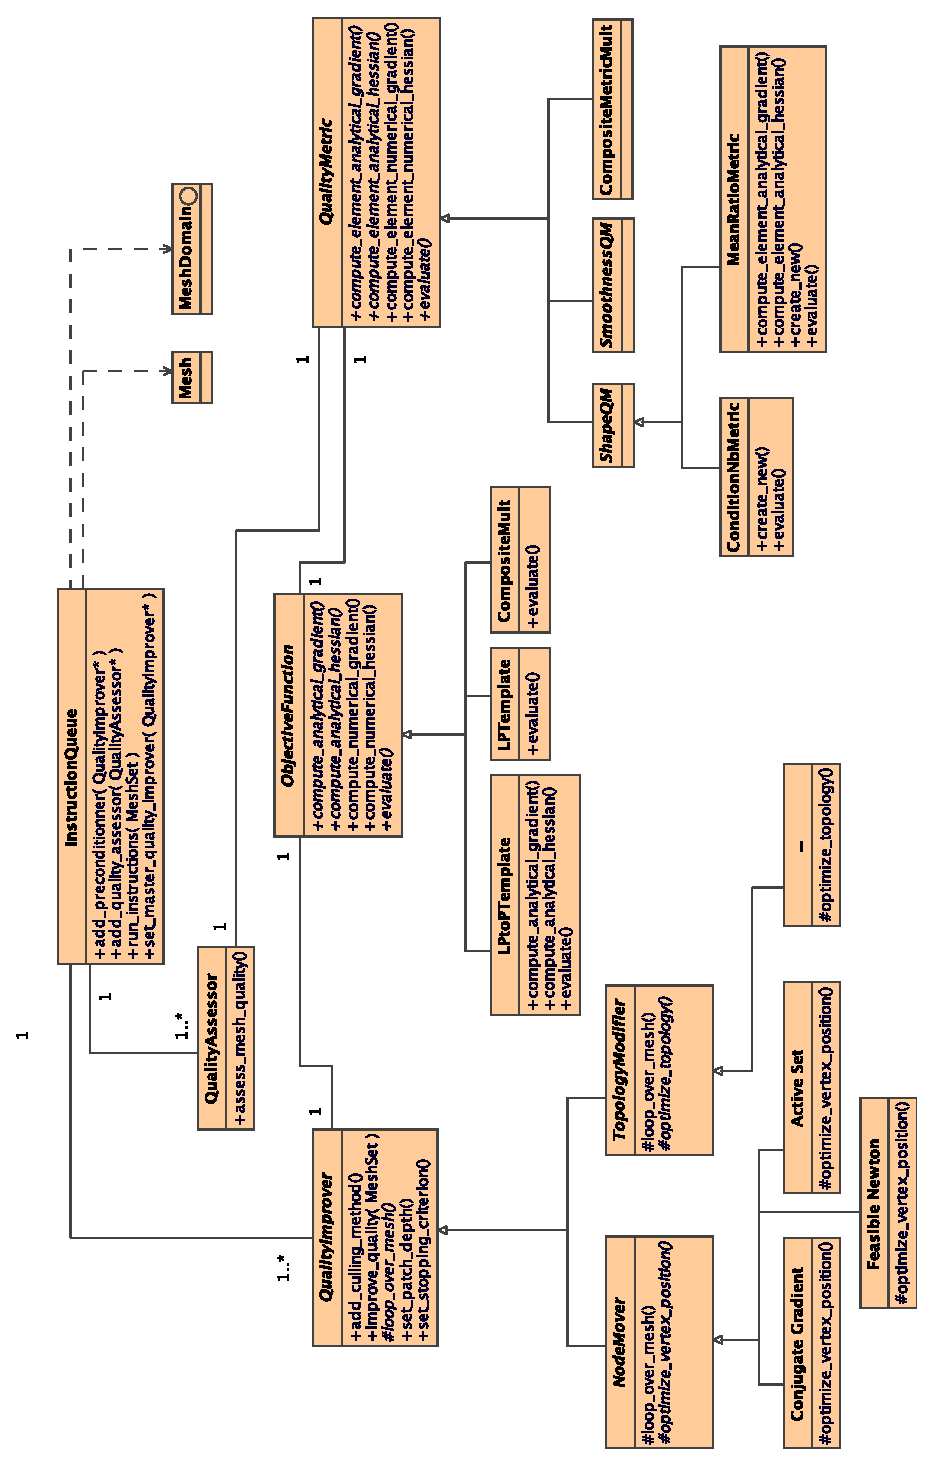
\includegraphics{../developer/UML/MesquiteUI.eps}
    \caption{Mesquite user interface UML class diagram.  Abstract
             classes and virtual functions are in italic. Vertical
             links with a triangle indicate inheritance. Plain links
             indicate association. Protected functions are prefixed
             with '\#', public ones with '+' .}
    \label{fig:uml}
\end{center}
\end{figure*}

The Mesquite architecture, shown in Figure \ref{fig:uml}, closely
follows the abstractions defined by the mathematical framework 
to describe the optimization problem.
In particular, the core abstract classes needed to
define a mesh quality improvement algorithm are {\tt QualityMetric},
{\tt ObjectiveFunction} (which takes a {\tt QualityMetric} as
input), and {\tt QualityImprover} (which takes an {\tt ObjectiveFunction}
as input).

In addition, a number of other classes have been created to support
the needs of mesh quality improvement algorithms:
\begin{itemize}
\item {\tt QualityAssessor}: to provide an evaluation of mesh
quality using standard statistical procedures,
\item {\tt TerminationCriterion}: to customize the stopping criteria
used with a mesh quality improvement algorithm,
\item {\tt InstructionQueue}: to compose quality improvers and
quality assessors together to form efficient mesh quality improvement
and evaluation methods, and
\item {\tt MeshSet} and {\tt PatchData}: to provide the mechanisms
for managing the application mesh and geometry information and the
mesh sub-domains used in optimization procedures.
\end{itemize}

The Mesquite architecture uses as much dynamic polymorphism in the
form of inheritance and virtual functions as is possible without
degrading performance.  This allows developers to add new
functionality to Mesquite by inheriting from the appropriate abstract
class and implementing its interface (i.e. its abstract virtual
functions).  We note that the mesh entities, defined by class {\tt
MsqMeshEntity}, are the only exception in our architecture.  Mesh
entities, i.e. triangles, tetrahedrons, quadrangles and hexahedrons,
are implemented in a single class, without the use of dynamic
polymorphism, to eliminate the performance impact of runtime
resolution.

We describe the details of the core classes {\tt
QualityMetric}, {\tt ObjectiveFunction}, {\tt QualityImprover}, {\tt
TerminationCriterion}, {\tt QualityAssessor}, {\tt MeshSet}, {\tt
PatchData}, and {\tt InstructionQueue}.
In each case, we give details
of the design and discuss the functionality currently implemented in
Mesquite.

\subsection{The Quality Metric -- Objective Function -- Quality Improver Trio} \label{sec:trio}

In Mesquite, the \texttt{QualityMetric} class provides a measure of
the quality of individual mesh entities.  Quality metrics can evaluate
either element quality (for example, the mean ratio shape quality
metric) or vertex quality (for example, the sum of the adjacent edge
lengths squared can be used as a measure of vertex smoothness).  
The primary functionality associated with the {\tt QualityMetric}
class is the `evaluate' function which returns a single quality value
for a given mesh entity.

In addition to the quality metric function value, the {\tt
QualityMetric} class also provides the gradient and Hessian
information needed for many optimization algorithms.  Numerical
approximations of the gradient and Hessian are automatically provided
by the \texttt{QualityMetric} base class.  Users can optionally
implement analytical expressions which are potentially more
computationally efficient.  For example, in the case of the mean ratio
quality metric implementation, the analytic calculation is
approximately twice as fast as the numerical computation although this
improved efficiency often comes at a higher implementation cost.  The
cost of implementing the analytical gradients and Hessians can often
be alleviated, however, by the use of automatic differentiation tools
(for example, \cite{bischofadic}).

Mesquite also allows the user to scale metric values or combine
multiple metrics together to form a composite metric.  However, only
metrics which are evaluated on the same type of mesh entity can be
composed together.  That is, Mesquite does not allow element-based
metrics and vertex-based metrics to be added or multiplied together
because the result is not a meaningful measure of either element or
vertex quality.

While the \texttt{QualityMetric} class provides a way to evaluate the
properties of individual mesh entities, the \texttt{ObjectiveFunction}
class provides a way of combining those values into a single number
for the domain of the optimization problem.  This domain can either be
the entire mesh or a sub-mesh containing a subset of the free vertices.
For example, one available objective function template $f$ is the $\ell_{2}^2$
function which is the standard $\ell_{2}$ vector norm squared.  
Given an element-based quality metric $q$ and a mesh sub-domain $E$, the mesh 
quality objective function $\cal F$ would be the composition of the template
objective function and the quality metric function 
\begin{equation}
{\cal F}({\bf x}) = f \circ q({\bf x}) = \sum_{i \in E} (q_i({\bf x}))^2 \;\; .
\end{equation}

Given a \texttt{QualityMetric} $q$ and a mesh sub-domain $E$, the
\texttt{ObjectiveFunction} derived class computes the value of $\cal
F$ and, for $f$ and $q$ satisfying the appropriate smoothness
conditions, the mesh quality objective function's gradient and Hessian
with respect to the vertex positions.  As with {\tt QualityMetric},
Mesquite allows the gradient of $\cal F$ to be calculated either
analytically or numerically. Computing the gradient of $\cal F$
numerically is computationally expensive but requires only the quality
metric values.  If the gradient is calculated analytically, the the
first derivative of the template objective function $f'$ and the
quality metric gradient $\nabla q$ are both required.\footnote{The 
quality metric gradients $\nabla q$ can be provided either numerically 
or analytically.}
To obtain the gradient of ${\cal F}$, the chain rule is applied
\begin{equation}
\nabla {\cal F}({\bf x}) = \amalg_{i \in E} \left[ \nabla q_i({\bf x}) 
 (f' \circ q({\bf x}) ) \right] \;\; ,
\end{equation}
where $ f' \circ q({\bf x})$ is a scalar and $\amalg_{i \in E}$ denotes the
assembly over all the elements or vertices, for element-based or 
vertex-based quality metrics respectively.
Due to the significant advantages in computational
cost, analytical gradients have been implemented for all of the
continuously differentiable template objective functions in Mesquite.
Furthermore, an analytical Hessian calculation has been implemented
for the $\ell_p^p$ template objective function.  

%\begin{table}[htb]
%\begin{center}
%\begin{tabular}{|c|c|c|}
%\hline
%Function & Gradient & Hessian\\
%\hline
%$\ell_P^P$     & Ana./Num.&Ana.\\
%$\ell_P$       & Ana./Num.& Not Avail.\\
%$\ell_{\infty}$& Not Avail.& Not Avail.\\
%Comp. Add      & Ana./Num.& Not Avail.\\
%Comp. Mult.    & Ana./Num.& Not Avail.\\
%Scalar Add     & Ana./Num.& Not Avail.\\
%Scalar Mult.   & Ana./Num.& Not Avail.\\
%\hline
%\end{tabular}
%\label{current-objfunc}
%\caption{List of the current objective functions available within
%Mesquite.  With each function is a description of the types of
%gradient and Hessian information available (Analytical and/or Numerical
%or Not Available).}
%\end{center}
%\end{table}

Mesquite has four composite objective functions.  These are
composite add, composite multiply, composite scalar add, and
composite scalar multiply.  This combination allows users
to combine two objective functions by adding or multiplying
their respective values or to adjust a single objective function
by adding a scalar value or by multiplying by a scalar value.  
The user can adjust the objective function to modify the
optimization problem or to make the objective function value
more easily interpreted.  Scaling objective function values
is often useful when using a termination criterion based on the
objective function values. Unlike the quality metrics, 
two objective functions can be combined
even if the underlying quality metrics are defined on different entity
types.  That is, an objective function which operates on a vertex-based
quality metric can be added to an objective function which operates
on an element-based quality metric.  This structure allows the user
to have the maximum flexibility in defining an objective function with
which to measure the quality of a mesh.


{\it Available Template Objective Functions.}  Mesquite currently has objective
function templates for the standard $\ell_{P}$ (where $P$ is a
positive integer) and $\ell_{\infty}$ vector norms.  A separate
template is provided for $\ell_{P}^{P}$, a function which has some
nice properties including a sparse Hessian matrix.  All of Mesquite's
quality improvers are designed to minimize a given objective function.
For objective functions that need to be maximized ({\it e.g.} an
$\ell_{1}$ objective function using an inverted mean ratio metric),
the function value is multiplied by negative one to obtain the
equivalent minimization problem.


The mesh quality improvement algorithms are a crucial component of the
Mesquite framework.  The two main types of improvement schemes
designed into Mesquite are {\tt VertexMover} and {\tt
TopologyModifier} for vertex relocation or topology modification,
respectively.  These methods take as input an {\tt ObjectiveFunction}
and often make extensive use of the gradient (and sometimes the
Hessian) information provided therein.  When writing a new algorithm,
the concrete \texttt{QualityImprover} always acts on an
\texttt{ObjectiveFunction} pointer to retrieve the function value and
gradient for a certain mesh and concrete \texttt{ObjectiveFunction} /
\texttt{QualityMetric} combination.  Dynamic polymorphism ensures at
runtime that the correct evaluations are performed.

One important aspect of both vertex movers and topology modifiers is
the ability to seamlessly perform an optimization of a whole mesh or
to perform a sequence of optimizations on sub-patches of the mesh.
This behavior is chosen by the user at the \texttt{QualityImprover}
level with the \texttt{set\_patch\_type} function inherited from
\texttt{QualityImprover}'s parent class, \texttt{PatchDataUser}. The
implementation to gather the mesh information into the patch is
carried out by \texttt{MeshSet} and \texttt{PatchData}, so that the
optimization algorithm receives the appropriate patch to improve
simply by inheriting from \texttt{QualityImprover}.  If needed, one can 
override the \texttt{set\_patch\_type} function to accept only specific
patch types.

A new quality improver is defined by inheriting from either the
\texttt{VertexMover} or the \texttt{TopologyModifier} abstract class.
Both classes are intermediate abstract classes inheriting from the
\texttt{QualityImprover} class (see Figure \ref{fig:uml}).  Their
essential functionality is to implement the \texttt{loop\_over\_mesh}
virtual function which shields the optimization algorithm developer
from the need to distinguish between local or global patches.  The
{\tt VertexMover} base class also checks the outer termination
criterion to stop iterating over mesh subsets (see section
\ref{termination_section}) and updates the application mesh after
optimizing a patch.

{\it Available Quality Improvement Algorithms.}  There are currently
three major concrete optimization algorithms implemented as {\tt VertexMover}s
in Mesquite: the conjugate gradient algorithm, the feasible Newton
algorithm, and the active set algorithm. The optimization of mesh
topology has been accounted for in the architecture, but no
implementation is available yet (i.e. no concrete
\texttt{TopologyModifier} class exists yet).


\subsection{Termination Criterion}
\label{termination_section}

Mesquite's \texttt{TerminationCriterion} class contains functionality
to customize the termination of the mesh quality improvement process.
As mentioned previously, many quality improvement algorithms can
perform mesh optimization on either the global mesh or on sub-meshes.
In the latter case, the algorithm must be capable of determining when
to terminate two processes: 1) the optimization on the sub-mesh and 2)
the iteration over the sub-meshes.  Mesquite's
\texttt{TerminationCriterion} class has been designed to handle either
of these cases.  Therefore, in general, quality improvers use two
\texttt{TerminationCriterion} objects: one, called the {\it inner
criterion}, to terminate the optimization of the sub-domain and
another, called the {\it outer criterion}, to terminate the iteration
over the sub-meshes.  Typically, quality improvers that support both
local and global optimizations always use two termination criterion. 
The outer criteria is set to terminate the optimization process after
one iteration in the global case.

{\it Available Termination Criterion.}  A wide range of cost, quality, 
and progress-centric termination
criterion types have been studied. These criteria have two basic types - 
absolute or relative - depending on whether or not the criterion is scale 
dependent.  Fourteen of these have been
implemented in \texttt{TerminationCriterion}.  Among the implemented
types are criteria which terminate optimization procedures due to
exceeding a set number of iterations, exceeding an allotted amount of
time, or reaching a mesh with a sufficiently small objective function
gradient.  Any combination of the available criteria can be set on a given
\texttt{TerminationCriterion} object.  Compound criteria types consist
of statements joined by 'OR', for which 
the optimization process will be terminated when {\it any} of
the criteria have been satisfied.  Currently we have found little use
for compound criteria joined by 'AND', but this also could be implemented. 

\subsection{Quality Assessors}

Mesquite's \texttt{QualityAssessor} class encapsulates functionality to
evaluate quality metric values for a given mesh, to accumulate
statistical information about those values, and to report that data to
the user.  In particular, a \texttt{QualityAssessor} object takes a
{\tt QualityMetric} class as input to evaluate a given mesh and then
reports information like the maximum, average, and standard deviation
of those values.

% \subsubsection{Culling Capabilities} \label{sec:culling}
% Mesquite includes methods called {\it culling} schemes
% which are intended to decrease the time it takes for the
% quality improvers to reach an adequate mesh.  These schemes
% the mporarily fix the positions of certain vertices which
%satisfy a given culling criteria.  These fixed vertices
%are said to be {\it culled} from the optimization procedure.
%This reduces the number of variables in the optimization
%problem, and therefore this modified problem can often
%be solved in significantly less time than the original problem.  
% LAF - there are no details here - it's not worth including as is

\subsection{Mesh Data Classes} \label{sec:MeshData}

There are two mesh data classes in Mesquite, \texttt{MeshSet} and
\texttt{PatchData}, which have been designed to meet two different
needs.  The {\tt MeshSet} class is a container that holds pointers, or
handles, to the meshes provided by the application.  It also provides
the mechanisms necessary to obtain the mesh information from the
application through a well-defined, flexible API (see Section
\ref{sec:meshset}).  To minimize the memory footprint of the Mesquite
library, only detailed information for the optimization procedure
subdomains is stored at any given time in the {\tt PatchData} class.
One or more {\tt PatchData} objects can be originated from the {\tt
MeshSet} object, and {\tt PatchData} obtains detailed mesh
information, such as vertex coordinates and element connectivity,
through the MeshSet accessor functionality.  The \texttt{PatchData}
class makes Mesquite scalable in that prohibitive memory costs
associated with making a copy of a large application mesh can be
avoided by dividing the mesh into patches on which to perform the
optimization sequentially.

\subsubsection{MeshSet Interactions with Application Meshes}
\label{sec:meshset}

\subsubsection{PatchData Interactions with QualityImprovers}

Quality improvers are written to relocate nodes or modify topology
within a \texttt{PatchData}, without any need to know whether the
\texttt{PatchData} corresponds to the whole mesh or a subset of
it. The \texttt{PatchData} information is generated by the
\texttt{MeshSet} class with the \texttt{get\_next\_patch} function ---
the equivalent of an iterator over a series of patches covering the
mesh.  The user can set Mesquite to use different types of
\texttt{PatchData}, ranging from a patch of elements containing one
particular vertex to a patch of vertices connected to a central vertex
through edges or a unique patch that covers the whole MeshSet
(recall that this could be the union of several meshes added by the
application to \texttt{MeshSet}).

\texttt{PatchData} and its associated classes
(e.g. \texttt{PatchDataVerticesMemento}) provides much functionality
to the optimization algorithms.  Memento patterns can remember the
state of a \texttt{PatchData} geometry or topology at a given
iteration and restore the \texttt{PatchData} to that state
later. Simple functions can move the \texttt{PatchData} $n$ vertices
in a direction $d \in \Bbb{R}^{3n}$ while constraining the boundary
vertices to their geometrical surface.

\subsection{The Instruction Queue} \label{sec:IQ}

The \texttt{InstructionQueue} class allows a sequence of operations
such as quality assessment and quality improvement to be performed on
a \texttt{MeshSet} object. The {\tt
InstructionQueue} provides a convenient framework to shield the user
from the algorithm syntax and to ensure a consistent use of the
Mesquite capabilities.  One or more quality improvers can be
associated with an {\tt InstructionQueue}, but one must be designated
as the {\it master} quality improver that determines the ultimate 
improvement goal.  All progress made by Mesquite will be
measured against the quality metrics set in the master quality
improver.  To improve the effectiveness and efficiency of the mesh
quality improvement process, several quality improvers can be used as
'pre-conditioners' for the master quality improver.  For example, a
user may precede an optimization-based master quality improver with a
mesh untangler and/or Laplacian smoothing.

Some predefined {\tt InstructionQueue} objects, called \emph
{wrappers}, are available for high-level or novice users. Those
typically consist of a quality assessor, followed by a mesh
pre-conditioner such as an untangler, followed by a master quality
improver, and finally another quality assessor.  Once an
InstructionQueue has been defined, a single call to {\tt
run\_instructions} will perform all the contained operations.  We note
that once an {\tt InstructionQueue} has been defined, it can be used
for several \texttt{MeshSet} objects.


\section{Telling Mesquite About Your Mesh}
\label{sec:meshes}

Mesquite is responsible for gathering information from the
application's mesh and geometry.  Because this must be as efficient as
possible, considerable attention has been given to the interface
between Mesquite and the application code.  Because Mesquite is
designed as a library to work on a broad assortment of mesh and
element types on complex geometrical domains, a general,
data-structure neutral API is needed.  In general, Mesquite requires
access to basic information about the mesh such as the number of
vertices and elements in the mesh, the vertex locations, and the
element connectivities.  To move the vertex locations, Mesquite needs
to set the vertex coordinate positions, and eventually, to perform
swapping operations Mesquite will need to add and delete various mesh
entities.  In addition, for smoothing meshes on complex surfaces,
access to operations on the underlying solid model such as normal
information and closest point information are required to ensure
vertices are constrained to the surface.

To expose this information, Mesquite defines a set of interfaces 
(C++ abstract base classes) that are specifically designed for mesh
quality improvement needs.  There are four such interfaces: Mesh,
VertexIterator, ElementIterator, and MeshDomain.
\begin{itemize}
\item {\it Mesh:} The Mesh interface represents the set of mesh
entities that are to be operated on.  It is through this interface
that one retrieves information about the mesh and its entities.
Examples of functionality provided by this interface include:
retrieving the number of elements in the mesh, determining which
elements contain a particular vertex, and modifying vertex
coordinates.
\item {\it VertexIterator:} The VertexIterator provides access to each
vertex in a mesh.  A VertexIterator is obtained from a Mesh object,
and is used to iterate through the list of all vertices in the Mesh
from which it was obtained.
\item {\it ElementIterator:} The ElementIterator provides access to
each element in a mesh.  Other than the type of entity it exposes, it
is identical to the VertexIterator.
\item {\it MeshDomain} The MeshDomain represents the set of geometric
domains to which the mesh may be constrained.  The MeshDomain
interface enables an application to restrict the locations to which a
vertex can be moved, such as constraining a vertex to a surface.
Through the MeshDomain interface, Mesquite's algorithms can also
obtain a domain's normal vector, which aides validity checking and 
decision making during the quality improvement process.
\end{itemize}
These interfaces are data-structure neutral and use only primitive
data types; an application may implement the Mesquite interfaces
without changing its existing mesh data structures.  Instead of
representing mesh entities with complex data structures or with typed
pointers, entities are identified with opaque values called handles.
Each mesh entity has a unique handle value, but otherwise handles have
no intrinsic meaning to Mesquite.  

Mesquite can instead use the mesh interfaces currently
being developed through the TSTT center.  This interface definition
effort focuses on providing access to information pertaining to low
level mesh objects such as vertices, edges, faces, and regions through
both array-based and iterator-based mechanisms.  It is designed to
support existing packages such as CUBIT, NWGrid, PAOMD, and Overture.
Considerations such as data neutrality, language interoperability
(achieved through use of the SIDL/Babel tools from LLNL \cite{babel}),
and achieving consensus within a large group of participants is
paramount (see \cite{Cubit-website}, \cite{overture}, \cite{aomd-imr},
and \cite{NWGrid-website}).  This interface definition effort is
evolving, and the Mesquite team is actively participating to ensure
that our needs for mesh quality improvement are adequately and
efficiently addressed.  A TSTT-based implementation of the Mesquite
interfaces will be available soon.  As such, any tool that exposes its
mesh through the TSTT interfaces can be used with Mesquite without
additional development.

The Mesquite-specific interfaces described above are fully compatible
with the current TSTT mesh and geometry interfaces, and in fact,
Mesquite's approach to data structure neutrality is directly derived
from the TSTT interfaces.  Although similar in spirit to the TSTT
interface, the Mesquite-specific interface is not as general, and 
therefore consist of fewer
functions and does not require additional tools such as Babel.

\subsection{The Simplified Geometry Engine}
\label{sec:geometry}

\subsection{Linking Mesquite with the TSTT Mesh Interface} 
\label{sec:TSTT}

\subsection{Implementing the Mesquite Mesh Interface}

Most users will want to skip this section and avoid the associated work. There are several manners
to give the mesh data to Mesquite, and implementing the Mesquite mesh interface is the one that
requires the most coding work. 

Let's review the alternative in the first place. For very simple meshes, Mesquite has an integrated
mesh database that can read in mesh files in specific format, such as VTK (see section \ref{sec:}). 
On the other hand, Mesquite is compatible with the TSTT mesh interface: this means that if you are
running a code that has implemented the TSTT mesh interface, you can link Mesquite with your code
and perform all mesh improvements through the TSTT mesh interface (see section \ref{sec:TSTT}).
Implementing the TSTT mesh interface also has the advantage that your code will be compatible with
the TSTT mesh interface standard: this is a very good investment. 

If you want to implement the specific Mesquite mesh interface, you probably have very specific
reasons in mind ... and you know what you are doing. In this section, we will give you the
documentation for the abstract classes. This will allow you to implement the interface. 


\section{Simplified Application Programming Interface}
\label{sec:wrappers}
To improve meshes with a minimum of Mesquite function calls, we have 
provided a set of wrapper classes that encapsulate the 
most commonly used combination of quality metrics, improvement
algorithms and stopping criterion. Essentially, the wrappers are
inherited from the InstructionQueue, setting in their constructors
which algorithms to call. Using these wrappers, only
two lines of code are required to improve a \texttt{MeshSet}.

For example, the \texttt{ShapeImprovementWrapper} class 
first uses the mean ratio quality
metric to assess and report the quality of the mesh elements. It then
untangles the mesh if necessary and improves the mesh with the
feasible Newton algorithm applied to the composition of the mean ratio
quality metric with the $\ell_2^2$ objective function. Finally, the
mesh quality is assessed and reported again. 

Wrappers do not provide access to low-level 
features such as setting a specific
termination criterion.  


\section{Detailed Application Programming Interface}

\subsection{Quality Metric}

{\it 
What is a quality metric? Define full range, acceptable range, what is means 
if the metric uses a map, nodal-invariance, well-posed metrics, averaging 
methods, sample points. Give a list of the individual metrics we support. 
Provide a key to the tables.
}

To implement a new quality metric, a user must inherit from the base
{\tt QualityMetric} class and implement the `evaluate' function.
{\tt QualityMetric} provides a wide range of
functionality that allows the quality metrics to be defined in a
flexible way and therefore gives the user the ability to modify the
metric in a variety of ways.  For example, the condition number
quality metric for a quadrilateral or hexahedral element is computed
by evaluating the condition number at a number of sample points in the
element.  Mesquite allows the user to select which set of sample
points are used in this calculation ({\it e.g.}, the element's
vertices) and how these values are combined to form a single metric
value ({\it e.g.}, linear averaging).  Mesquite is currently being
extended to allow certain quality metrics to be referenced to a
non-isotropic element.

{\it Currently Available Quality Metrics.}  Quality metrics within
Mesquite are grouped by the type of mesh properties that they measure.
Currently, there are four property groups: shape, smoothness, volume,
and untangle.  Composite metrics which allow the user to combine
multiple metrics or to scale metrics are given a separate group,
composite.  Future Mesquite development will include the
implementation of metrics falling under other group headings such as
orthogonality, shear, and alignment.  Table \ref{current-metrics}
lists the quality metrics currently available within Mesquite.  For
detailed definitions of the metrics, see \cite{Kn01}.  We note that
the implementation of the mean ratio metric has been extensively
optimized, and analytical gradients and Hessians are available for
that function.  Other metrics currently use numerical gradients and
Hessians.

The two composite metrics which are currently implemented
allow users to either multiply two metrics' values
together or raise a single metric's value to a given power.
The latter allows for negative powers and can therefore be used
to obtain the inverse of any Mesquite quality metric.  

\begin{table*}[htb]
\begin{center}
\begin{tabular}{|l|c|c|c|c|}
\hline
Metric & Group & Mesh Type & Feasibility Region &Entity Type\\
\hline
Area Smoothness &Smoothness & Any & No & Elements\\
Aspect Ratio & Shape &Tri/Tet & No & Elements\\
Composite Mult. & Composite &Any& Yes/No & Either\\
Composite Power & Composite &Any& Yes/No & Either\\
Cond. Num.& Shape & Any & Yes & Elements \\
Corner Jacobian & Volume & Any & No & Elements \\
Edge Length &Smoothness & Any & No & Vertices \\
Edge Length Range & Smoothness & Any &No & Vertices\\
Mean Ratio &Shape & Any & Yes &Elements\\
Untangle Beta &Untangle &Any&Yes&Elements\\
Vert. Cond. Num.& Shape & Any & Yes & Vertices\\
\hline
\end{tabular}
\label{current-metrics}
\caption{List of the current Mesquite quality metrics. The table also
indicates the metric group, the mesh types for which the metric is
valid, whether the metric is only valid within a feasible
region, and the type of entity for which the metric is defined (elements
or vertices).  Note that there may be a feasible region for composite
metrics depending on whether the underlying metrics require such a
constraint.}
\end{center}
\end{table*}


\begin{table}[h]
\begin{center}
\begin{tabular}{|l|c|c|c|c|c|}
\hline
Metric Name & Type & Dimension & Full Range & Ideal & Degenerate \\ \hline
Inverse Mean Ratio & Shape & 2D, 3D & $[0,1]$ & 1 & 0 \\ 
Mean Ratio &  &  &  &  &  \\ 
Condition Number &  &  &  &  &  \\ 
Untangle &  &  &  &  &  \\ 
Aspect Ratio Gamma &  &  &  &  &  \\ 
\hline
\end{tabular}
\caption{\label{QualityMetrics1} Mesquite Quality Metrics Summary, Part I}
\end{center}
\end{table}

\begin{table}[h]
\begin{center}
\begin{tabular}{|l|c|c|c|c|c|c|}
\hline
Metric Name & Map? & Averaging & Sample Pts & Elements & Gradient & Source \\ \hline
Inverse Mean Ratio & No & Harmonic & Vertices & TQTH & Analytic & \\ 
Mean Ratio &  &  &  &  &  \\ 
Condition Number &  &  &  &  &  \\ 
Untangle &  &  &  &  &  \\ 
Aspect Ratio Gamma &  &  &  &  &  \\ 
\hline
\end{tabular}
\caption{\label{QualityMetrics2} Mesquite Quality Metrics Summary, Part II}
\end{center}
\end{table}

\noindent {\bf Mean Ratio Metric} \newline
Give description, formulas. 

\subsection{Objective Function}
List of all the templates. What is the difference between a template and
an objective function? For each element of the mesh (or for each 
free-node of the mesh), let there be an associated quality metric, 
$\mu_m$.  Define the vector 
\begin{equation}
{\bf U} = [ \mu_1, \mu_2, \ldots, \mu_M ]
\end{equation}
where $M$ is the number of elements or free-nodes in the mesh. \newline

\noindent Available templates in Mesquite: \newline

\noindent {\bf The $\ell_p$ Template} \newline
Given $1 \leq p < \infty$, let
\begin{equation}
\| {\bf U} \|_p = ( \sum_{m=1}^M \mid \mu_m \mid^p )^{1/p}
\end{equation}
be the $\ell_p$ template. \newline

\noindent {\bf The $\ell_p^p$ Template} \newline
Given $1 \leq p < \infty$, let $\| {\bf U} \|_p^p$ be the 
$\ell_p^p$ template. \newline

\noindent {\bf The $\ell_{\infty}$ Template} \newline
The $\ell_{\infty}$ template is
\begin{equation}
\| {\bf U} \|_{\infty} = \max_{m=1,\ldots,M} \mid \mu_m \mid
\end{equation}

These are currently the only templates available in Mesquite.
We soon hope to add the 'max' template:
\begin{equation}
MAX = \max_{m=1,\ldots,M} ( \mu_m )
\end{equation}

Which of these templates has numerical/analytic gradient/Hessian?

\subsection{Vertex Mover}
List solvers and appropriate templates. Is a solver the same things as a 
vertex mover? List options.

\begin{table}[h]
\begin{center}
\begin{tabular}{|l|c|c|c|c|c|}
\hline
Solver Name & Description & Templates & L/G & Num/Anal & Fixed Vertices? \\ \hline
Steepest Descent & Classical & $\ell_p$ & Both & Both & Yes \\
Conjugate Gradient & & & & & \\
Feasible Newton & & & & & \\
Active Set & & Own & & & \\
Laplace & & None & & & \\
Randomize & & None & & & \\
\hline
\end{tabular}
\caption{\label{Solvers} Mesquite Solver Summary}
\end{center}
\end{table}


\subsection{Topology Modifier}

\subsection{Termination Criteria}
List, along with uses.

\subsection{Culling Algorithms}

\subsection{Quality Assessment}

\subsection{Instruction Queue}
Setting the master quality improver, setting up and using preconditioners,
using quality assessors, running the instruction queue.

\subsection{Composite Metrics}

\subsection{Composite Objective Functions}
The only ones currently available are CompositeMult, CompositeAdd,
CompositeScalarMult, and CompositeScalarAdd.



\section{Hints for Performance Profiling}
Compiler options, aggregation.

\chapter{Extending Mesquite}

\section{Mesquite Programming Framework}

\subsection{Directory Structure}

The base directory of the Mesquite project contains several
sub-directories which are intended to help keep the project's
files organized.  Some of the sub-directories themselves are
also sub-divided.  Below are descriptions of the first level
of sub-directories ({\it i.e.,} the directories contained in the
base directory).
\begin{enumerate}
\item doc:  Contains a version of this document and a version of
the developer's documentation generated with doxygen (TODO: acknowledge
doxygen).
\item external:  Contains directories which can be used to store external
libraries.  These libraries are not necessarily provided with Mesquite.
\item include:  Contains the Mesquite header file, ``Mesquite.hpp.''
\item includeLinks:  Contains soft links to the other header files
used within Mesquite.  
\item lib:  The location where the Mesquite library, ``libmesquite.a,'' is
stored.
\item meshFiles:  Contains example meshes that are used in some of
the test cases.
\item mswindow:  Contains the project file for compiling with Visual C++
(TODO: VC++ trademark statement???).
\item obj:  The directory where the object files are placed.
\item src:  Contains the Mesquite source code and header files (except for
Mesquite.hpp).
\item testSuite:  Contains example driver codes which use Mesquite.  These
test cases can only be ran when linked with the correct libraries (generally,
AOMD or MDB).
\item TSTT-interface:  Contains the copy of the TSTT header file,
``TSTT\_Base.h,'' which is compatible with Mesquite.
\end{enumerate}

\subsection{Code Testing Framework}

Another integral part of the Mesquite framework is the code testing
infrastructure.  Several testing methodologies have been included
within Mesquite. Unit testing is extensively used to facilitate
development and ensure low-level robustness. Functional testing is
used to ensure that user case scenarios run smoothly.

We use a broad definition for unit tests in Mesquite. Any test
performed on a class without need for the entire Mesquite framework is
considered a unit test. This encompasses simple assertions like
checking the result of the multiplication of a matrix $A \in
\Bbb{R}^{3 \times 3}$ by a vector $v \in \Bbb{R}^{3}$ to more complex
assertions such as checking that a concrete \texttt{QualityImprover}
correctly repositions a free vertex in a simple patch for a given
objective function and quality metric.

Mesquite uses a readily available testing framework called CppUnit
\cite{cppunit} --- essentially the well known jUnit testing framework
ported to C++.  Using the unit testing methodology allows the
developers to write far more robust code.

Applications using Mesquite may also find the testing framework useful
when verifying their additions to the code. In particular,
applications that prefer to implement Mesquite's mesh interface
instead of using the TSTT mesh interface will want to
check their implementation with the corresponding unit test collection
available in Mesquite. In addition, analytic gradient and Hessian
implementations can be checked against the numerical version provided
by the {\tt QualityMetric} base class using readily available unit
tests.

In addition to unit tests, the Mesquite test suite also includes
a range of functional tests.  While these tests also use the
CppUnit framework, they differ from unit tests in that 
functional tests require the entire Mesquite framework.
The functional tests are complete and often complex mesh
optimization problems.  These tests are intended to ensure that
the individual units of the Mesquite code work together correctly.
Performing these tests not only helps
validate the code but also allows developers to evaluate the
effects of code modifications in terms of Mesquite's accuracy
and efficiency on `real world' problems.

\section{Creating a New Quality Metric}

\section{Creating a New Objective Function}

\section{Creating a New Vertex Mover Algorithm}

\section{Creating a New Topology Modifier Algorithm}


\chapter{Troubleshooting}

\chapter{Caveats, Limitations, and Disclaimers}

\chapter{User Support}

{\it Mailing lists, web site, examples, tutorials (pointer to slides?), 
instructions on downloading the software (open source, preparing 
derivative works), referencing Mesquite.}

\chapter{The Mesquite Team}

The core Mesquite team consists of five people from Sandia
National Laboratories (SNL) and Argonne National Laboratory (ANL):
Micheal Brewer (SNL), Lori Freitag (Co-PI, SNL), Patrick Knupp (Co-PI, SNL), 
Thomas Leurent (ANL), and Darryl Melander (SNL).  In addition,
significant contributions to the software have been made by
Todd Munson (ANL) who developed the Feasible Newton Solver.

\chapter{The Mesquite Development Plan}

{\it Timeline for proposed additions to the software.}



\chapter{Appendices}

\section{Appendix A: Mesh Interface}
\label{append_mesh}

\newcommand{\entrylabel}[1]{
   {\parbox[b]{\labelwidth-4pt}{\makebox[0pt][l]{\textbf{#1}}\\}}}
\newenvironment{Desc}
{\begin{list}{}
  {
    \settowidth{\labelwidth}{40pt}
    \setlength{\leftmargin}{\labelwidth}
    \setlength{\parsep}{0pt}
    \setlength{\itemsep}{-4pt}
    \renewcommand{\makelabel}{\entrylabel}
  }
}
{\end{list}}

\subsection{Detailed Description}
A Mesquite::Mesh is a collection of mesh elements which are composed of mesh vertices. Intermediate objects are not accessible through this interface (where intermediate objects include things like the faces of a hex, or an element's edges).

\subsection{Member Function Documentation}
\index{Mesquite::Mesh@{Mesquite::Mesh}!element_get_attached_vertex_count@{element\_\-get\_\-attached\_\-vertex\_\-count}}
\index{element_get_attached_vertex_count@{element\_\-get\_\-attached\_\-vertex\_\-count}!Mesquite::Mesh@{Mesquite::Mesh}}
\subsubsection{\setlength{\rightskip}{0pt plus 5cm}virtual size\_\-t Mesquite::Mesh::element\_\-get\_\-attached\_\-vertex\_\-count (Element\-Handle {\em elem}, {\bf Msq\-Error} \& {\em err}) honest\hspace{0.3cm}{\tt  [pure virtual]}}\label{classMesquite_1_1Mesh_a17}


Gets the number of vertices in this element. This data can also be found by querying the element's topology and getting the number of vertices per element for that topology type. 

\index{element_get_attached_vertex_indices@{element\_\-get\_\-attached\_\-vertex\_\-indices}!Mesquite::Mesh@{Mesquite::Mesh}}
\subsubsection{\setlength{\rightskip}{0pt plus 5cm}virtual void Mesquite::Mesh::element\_\-get\_\-attached\_\-vertex\_\-indices (Element\-Handle {\em element}, size\_\-t $\ast$ {\em index\_\-array}, size\_\-t {\em array\_\-size}, {\bf Msq\-Error} \& {\em err})\hspace{0.3cm}{\tt  [pure virtual]}}\label{classMesquite_1_1Mesh_a19}


Identifies the vertices attached to this element by returning each vertex's global index. The vertex's global index indicates where that element can be found in the array returned by {\bf Mesh::get\_\-all\_\-vertices}. 

\index{element_iterator@{element\_\-iterator}!Mesquite::Mesh@{Mesquite::Mesh}}
\subsubsection{\setlength{\rightskip}{0pt plus 5cm}virtual Element\-Iterator$\ast$ Mesquite::Mesh::element\_\-iterator ({\bf Msq\-Error} \& {\em err})\hspace{0.3cm}{\tt  [pure virtual]}}\label{classMesquite_1_1Mesh_a6}


Returns a pointer to an iterator that iterates over the set of all top-level elements in this mesh. The calling code should delete the returned iterator when it is finished with it. If elements are added or removed from the {\bf Mesh} after obtaining an iterator, the behavior of that iterator is undefined. 

\index{elements_get_attached_vertices@{elements\_\-get\_\-attached\_\-vertices}!Mesquite::Mesh@{Mesquite::Mesh}}
\subsubsection{\setlength{\rightskip}{0pt plus 5cm}virtual void Mesquite::Mesh::elements\_\-get\_\-attached\_\-vertices (Element\-Handle $\ast$ {\em elem\_\-handles}, size\_\-t {\em num\_\-elems}, Vertex\-Handle $\ast$ {\em vert\_\-handles}, size\_\-t \& {\em sizeof\_\-vert\_\-handles}, size\_\-t $\ast$ {\em csr\_\-data}, size\_\-t \& {\em sizeof\_\-csr\_\-data}, size\_\-t $\ast$ {\em csr\_\-offsets}, {\bf Msq\-Error} \& {\em err})\hspace{0.3cm}{\tt  [pure virtual]}}\label{classMesquite_1_1Mesh_a18}


Returns the vertices that are part of the topological definition of each element in the \char`\"{}elem\_\-handles\char`\"{} array.

When this function is called, the following must be true:\begin{enumerate}
\item 
\char`\"{}elem\_\-handles\char`\"{} points at an array of \char`\"{}num\_\-elems\char`\"{} element handles.\item 
\char`\"{}vert\_\-handles\char`\"{} points at an array of size \char`\"{}sizeof\_\-vert\_\-handles\char`\"{}\item 
\char`\"{}csr\_\-data\char`\"{} points at an array of size \char`\"{}sizeof\_\-csr\_\-data\char`\"{}\item 
\char`\"{}csr\_\-offsets\char`\"{} points at an array of size \char`\"{}num\_\-elems+1\char`\"{}\end{enumerate}
When this function returns, adjacency information will be stored in csr format:\begin{enumerate}
\item 
\char`\"{}vert\_\-handles\char`\"{} stores handles to all vertices found in one or more of the elements. Each vertex appears only once in \char`\"{}vert\_\-handles\char`\"{}, even if it is in multiple elements.\item 
\char`\"{}sizeof\_\-vert\_\-handles\char`\"{} is set to the number of vertex handles placed into \char`\"{}vert\_\-handles\char`\"{}.\item 
\char`\"{}sizeof\_\-csr\_\-data\char`\"{} is set to the total number of vertex uses (for example, sizeof\_\-csr\_\-data = 6 in the case of 2 TRIANGLES, even if the two triangles share some vertices).\item 
\char`\"{}csr\_\-offsets\char`\"{} is filled such that csr\_\-offset[i] indicates the location of entity i's first adjacency in \char`\"{}csr\_\-data\char`\"{}. The number of vertices in element i is equal to csr\_\-offsets[i+1] - csr\_\-offsets[i]. For this reason, csr\_\-offsets[num\_\-elems] is set to the new value of \char`\"{}sizeof\_\-csr\_\-data\char`\"{}.\item 
\char`\"{}csr\_\-data\char`\"{} stores integer offsets which give the location of each adjacency in the \char`\"{}vert\_\-handles\char`\"{} array.\end{enumerate}
As an example of how to use this data, you can get the handle of the first vertex in element \#3 like this: 

\footnotesize\begin{verbatim}VertexHandle vh = vert_handles[ csr_data[ csr_offsets[3] ] ] 
\end{verbatim}\normalsize 


and the second vertex of element \#3 like this: 

\footnotesize\begin{verbatim}VertexHandle vh = vert_handles[ csr_data[ csr_offsets[3]+1 ] ] 
\end{verbatim}\normalsize 
 

\index{elements_get_topologies@{elements\_\-get\_\-topologies}!Mesquite::Mesh@{Mesquite::Mesh}}
\subsubsection{\setlength{\rightskip}{0pt plus 5cm}virtual void Mesquite::Mesh::elements\_\-get\_\-topologies (Element\-Handle $\ast$ {\em element\_\-handle\_\-array}, Entity\-Topology $\ast$ {\em element\_\-topologies}, size\_\-t {\em num\_\-elements}, {\bf Msq\-Error} \& {\em err})\hspace{0.3cm}{\tt  [pure virtual]}}\label{classMesquite_1_1Mesh_a21}


Returns the topologies of the given entities. The \char`\"{}entity\_\-topologies\char`\"{} array must be at least \char`\"{}num\_\-elements\char`\"{} in size. 

\index{get_all_elements@{get\_\-all\_\-elements}!Mesquite::Mesh@{Mesquite::Mesh}}
\subsubsection{\setlength{\rightskip}{0pt plus 5cm}virtual void Mesquite::Mesh::get\_\-all\_\-elements (Element\-Handle $\ast$ {\em elem\_\-array}, size\_\-t {\em array\_\-size}, {\bf Msq\-Error} \& {\em err})\hspace{0.3cm}{\tt  [pure virtual]}}\label{classMesquite_1_1Mesh_a4}


Fills array with handles to all elements in the mesh.

\begin{Desc}
\item[Parameters: ]\par
\begin{description}
\item[{\em 
array\_\-size}]Must be at least the number of elements. If less than the mesh number of elements, an error is set (and a partial copy is made). \end{description}
\end{Desc}


\index{get_all_vertices@{get\_\-all\_\-vertices}!Mesquite::Mesh@{Mesquite::Mesh}}
\subsubsection{\setlength{\rightskip}{0pt plus 5cm}virtual void Mesquite::Mesh::get\_\-all\_\-vertices (Vertex\-Handle $\ast$ {\em vert\_\-array}, size\_\-t {\em array\_\-size}, {\bf Msq\-Error} \& {\em err})\hspace{0.3cm}{\tt  [pure virtual]}}\label{classMesquite_1_1Mesh_a3}


Fills array with handles to all vertices in the mesh.

\begin{Desc}
\item[Parameters: ]\par
\begin{description}
\item[{\em 
array\_\-size}]Must be at least the number of vertices. If less than the mesh number of vertices, an error is set (and a partial copy is made). \end{description}
\end{Desc}


\index{release@{release}!Mesquite::Mesh@{Mesquite::Mesh}}
\subsubsection{\setlength{\rightskip}{0pt plus 5cm}virtual void Mesquite::Mesh::release ()\hspace{0.3cm}{\tt  [pure virtual]}}\label{classMesquite_1_1Mesh_a23}


Instead of deleting a {\bf Mesh} when you think you are done, call {\bf release()} {\rm (p.\,\pageref{classMesquite_1_1Mesh_a23})}. In simple cases, the implementation could just call the destructor. More sophisticated implementations may want to keep the {\bf Mesh} object to live longer than {\bf Mesquite} is using it. 

\index{release_entity_handles@{release\_\-entity\_\-handles}!Mesquite::Mesh@{Mesquite::Mesh}}
\subsubsection{\setlength{\rightskip}{0pt plus 5cm}virtual void Mesquite::Mesh::release\_\-entity\_\-handles ({\bf Entity\-Handle} $\ast$ {\em handle\_\-array}, size\_\-t {\em num\_\-handles}, {\bf Msq\-Error} \& {\em err})\hspace{0.3cm}{\tt  [pure virtual]}}\label{classMesquite_1_1Mesh_a22}


Tells the mesh that the client is finished with a given entity handle. 

\index{vertex_get_attached_element_count@{vertex\_\-get\_\-attached\_\-element\_\-count}!Mesquite::Mesh@{Mesquite::Mesh}}
\subsubsection{\setlength{\rightskip}{0pt plus 5cm}virtual size\_\-t Mesquite::Mesh::vertex\_\-get\_\-attached\_\-element\_\-count (Vertex\-Handle {\em vertex}, {\bf Msq\-Error} \& {\em err}) const\hspace{0.3cm}{\tt  [pure virtual]}}\label{classMesquite_1_1Mesh_a15}


Gets the number of elements attached to this vertex. Useful to determine how large the \char`\"{}elem\_\-array\char`\"{} parameter of the {\bf vertex\_\-get\_\-attached\_\-elements()} function must be. 

\index{vertex_get_byte@{vertex\_\-get\_\-byte}!Mesquite::Mesh@{Mesquite::Mesh}}
\subsubsection{\setlength{\rightskip}{0pt plus 5cm}virtual void Mesquite::Mesh::vertex\_\-get\_\-byte (Vertex\-Handle {\em vertex}, unsigned char $\ast$ {\em byte}, {\bf Msq\-Error} \& {\em err})\hspace{0.3cm}{\tt  [pure virtual]}}\label{classMesquite_1_1Mesh_a13}


Retrieve the byte value for the specified vertex or vertices. The byte value is 0 if it has not yet been set via one of the \_\-set\_\-byte() functions. 

\index{vertex_is_fixed@{vertex\_\-is\_\-fixed}!Mesquite::Mesh@{Mesquite::Mesh}}
\subsubsection{\setlength{\rightskip}{0pt plus 5cm}virtual bool Mesquite::Mesh::vertex\_\-is\_\-fixed (Vertex\-Handle {\em vertex}, {\bf Msq\-Error} \& {\em err})\hspace{0.3cm}{\tt  [pure virtual]}}\label{classMesquite_1_1Mesh_a7}

Returns true or false, indicating whether the vertex is allowed to be repositioned. True indicates that the vertex is fixed and cannot be moved. Note that this is a read-only property; this flag can't be modified by users of the Mesquite::Mesh interface. 

\index{vertex_is_on_boundary@{vertex\_\-is\_\-on\_\-boundary}!Mesquite::Mesh@{Mesquite::Mesh}}
\subsubsection{\setlength{\rightskip}{0pt plus 5cm}virtual bool Mesquite::Mesh::vertex\_\-is\_\-on\_\-boundary (Vertex\-Handle {\em vertex}, {\bf Msq\-Error} \& {\em err})\hspace{0.3cm}{\tt  [pure virtual]}}\label{classMesquite_1_1Mesh_a8}


Returns true or false, indicating whether the vertex is on the boundary. Boundary nodes may be treated as a special case by some algorithms or culling methods. Note that this is a read-only property; this flag can't be modified by users of the Mesquite::Mesh interface. 

\index{vertex_iterator@{vertex\_\-iterator}!Mesquite::Mesh@{Mesquite::Mesh}}
\subsubsection{\setlength{\rightskip}{0pt plus 5cm}virtual Vertex\-Iterator$\ast$ Mesquite::Mesh::vertex\_\-iterator ({\bf Msq\-Error} \& {\em err})\hspace{0.3cm}{\tt  [pure virtual]}}\label{classMesquite_1_1Mesh_a5}


Returns a pointer to an iterator that iterates over the set of all vertices in this mesh. The calling code should delete the returned iterator when it is finished with it. If vertices are added or removed from the {\bf Mesh} after obtaining an iterator, the behavior of that iterator is undefined. 

\index{vertex_set_byte@{vertex\_\-set\_\-byte}!Mesquite::Mesh@{Mesquite::Mesh}}
\subsubsection{\setlength{\rightskip}{0pt plus 5cm}virtual void Mesquite::Mesh::vertex\_\-set\_\-byte (Vertex\-Handle {\em vertex}, unsigned char {\em byte}, {\bf Msq\-Error} \& {\em err})\hspace{0.3cm}{\tt  [pure virtual]}}\label{classMesquite_1_1Mesh_a11}


Each vertex has a byte-sized flag that can be used to store flags. This byte's value is neither set nor used by the mesh implementation. It is intended to be used by {\bf Mesquite} algorithms. Until a vertex's byte has been explicitly set, its value is 0. 



\section{Appendix B: Conjugate Gradient Algorithm }
\label{append_conjgrad}
This algorithm requires only
the objective function value and the objective function gradient. 
In Mesquite this is usually done by applying the chain rule described in 
section \ref{objective_section} to the
analytical gradient of the objective function given the numerical or
analytical gradients of the elements. The conjugate gradient algorithm
has a linear convergence property for most problems. By using the
Polak-Ribi\`ere scheme to select a search direction which is a
combination of the gradient at the current iteration with the gradient
from one or more previous iteration, it avoids the zigzagging behavior
exhibited by the steepest descent algorithm when the equal cost
surfaces of the objective function are elongated (e.g. in narrow
valleys). In Mesquite this algorithm can be used with mesh patches of
any size; thus it is appropriate for optimizing all node positions 
simultaneously for any combination of $C^1$ objective functions and
quality metrics (see \cite{FeasNewt} for more details). 

\section{Appendix C: Feasible Newton Algorithm }
\label{append_feasnewt}
Newton's method minimizes a quadratic
approximation of a non-linear objective function. The algorithm requires
the objective function value, its gradient, \emph{and} its Hessian information.
Again, in Mesquite this
is usually done by computing the analytical gradient and Hessian of
the objective function given the numerical or analytical gradients and
Hessians of the quality metrics.  Note that objective functions that
lead to non-sparse Hessians entail a prohibitive memory cost in
Mesquite.\footnote{$\ell_p$ for $p \geq 2$ is such a function. The
number of variables in the objective function is the number of degrees
of freedom of the mesh, which must be squared to obtain the number of
entries in a dense Hessian.}  Newton's method is known to converge
super-linearly near a non-singular local minimum.   
Mesh-optimization problems that are performed within the neighborhood of
the minimum are a perfect application for Newton's method. In
Mesquite this algorithm can be used with mesh patches of any size,
making it appropriate to optimize all vertex positions simultaneously
for any $C^2$ objective function with a sparse Hessian.  In practice,
users will often observe an order of magnitude improvement in
computation time when using the feasible Newton algorithm instead of
the conjugate gradient algorithm, making feasible Newton a worthwhile
choice when applicable (see \cite{FeasNewt} for more details).

\section{Appendix D: Active Set Method }
\label{append_activeset}
The active set algorithm has been
developed for non-continuously differentiable objective functions such
as those computing the maximum value of a quality metric within a
patch of elements. This method is based on a non-smooth steepest
descent algorithm which efficiently computes a search direction and
step size based on the gradients of the values contained in the active
set.  Currently, this algorithm works on a patch of triangular or 
tetrahedral elements that 
contain a single free vertex.  Repeated
sweeps over the free vertices in the mesh leads to overall mesh
improvement (see \cite{fp:ijnme00} for more details).


\chapter{Acknowledgments}

Mesquite is supported under the DOE SciDAC Terascale Simulation 
Tools and Technology (TSTT) project \cite{tstt}.  

{\it Funding sources (DOE SciDAC Program, Chuck Romine), Related activities
(TSTT, Cubit, Opt-MS), helpful folks (RPI for AOMD, TSTT for MDB, LLNL
for Overture tests, etc.}


\bibliographystyle{plain}
\bibliography{mesquite}


\end{document}

